\documentclass{standalone}
\usepackage{tikz}
\usetikzlibrary{patterns, positioning}


\begin{document}
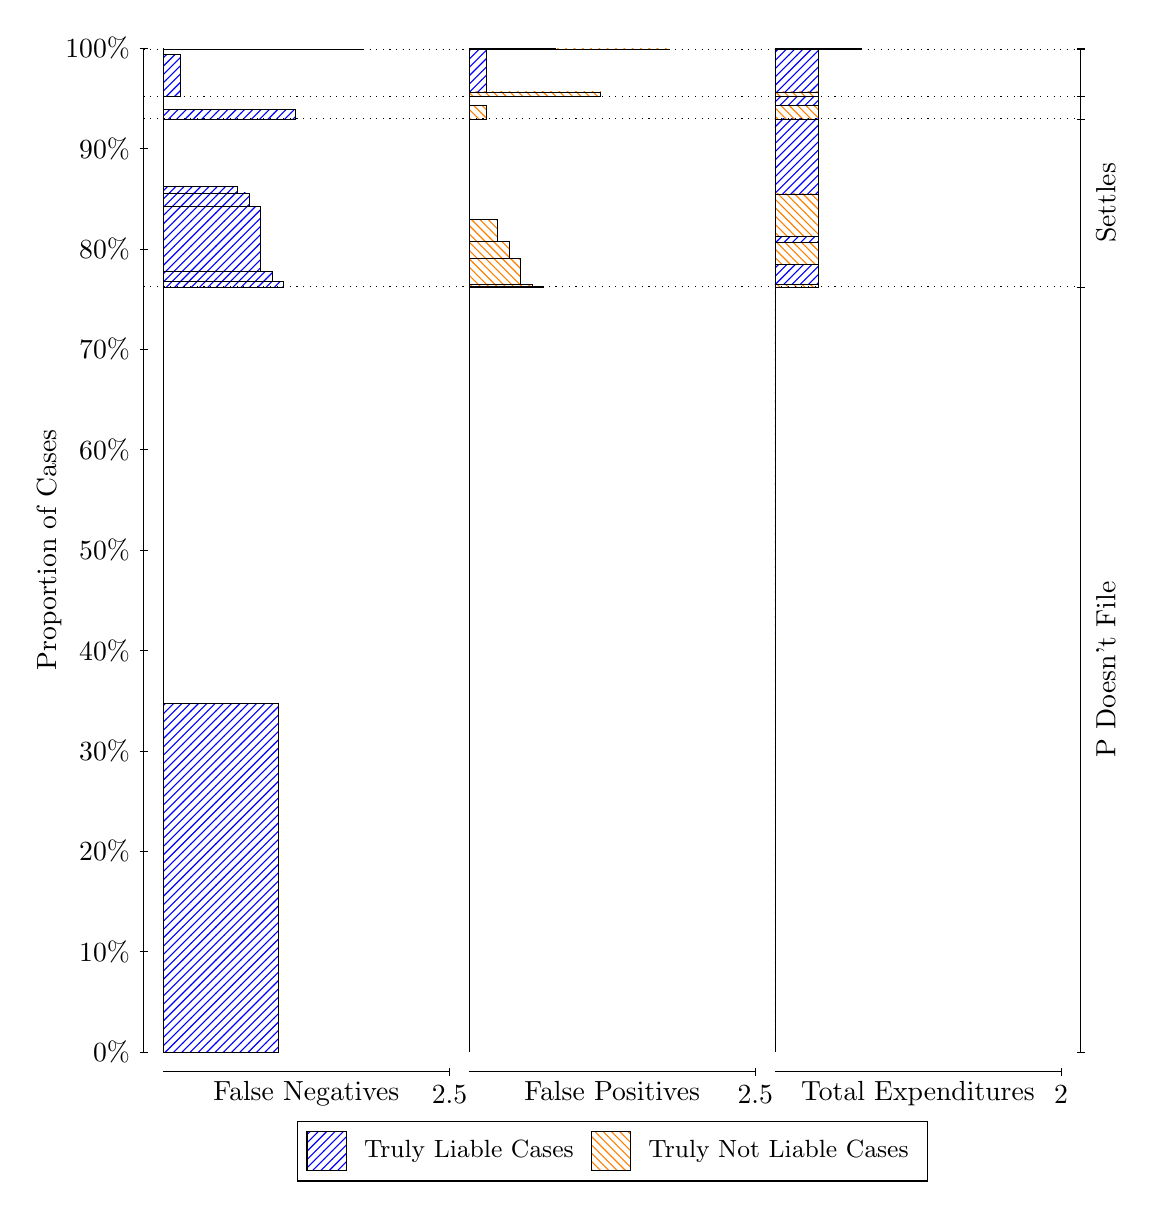
\begin{tikzpicture}
\draw[black, very thin] (1.5,1.75) -- (1.5,14.5);
\node[rotate=90, text=black, anchor=center] at (0.3, 8.125) {Proportion of Cases};
\draw[black, very thin] (1.45,1.75) -- (1.55,1.75);
\node[text=black, anchor=east] at (1.45, 1.75) {0\%};
\draw[black, very thin] (1.45,3.025) -- (1.55,3.025);
\node[text=black, anchor=east] at (1.45, 3.025) {10\%};
\draw[black, very thin] (1.45,4.3) -- (1.55,4.3);
\node[text=black, anchor=east] at (1.45, 4.3) {20\%};
\draw[black, very thin] (1.45,5.575) -- (1.55,5.575);
\node[text=black, anchor=east] at (1.45, 5.575) {30\%};
\draw[black, very thin] (1.45,6.85) -- (1.55,6.85);
\node[text=black, anchor=east] at (1.45, 6.85) {40\%};
\draw[black, very thin] (1.45,8.125) -- (1.55,8.125);
\node[text=black, anchor=east] at (1.45, 8.125) {50\%};
\draw[black, very thin] (1.45,9.4) -- (1.55,9.4);
\node[text=black, anchor=east] at (1.45, 9.4) {60\%};
\draw[black, very thin] (1.45,10.675) -- (1.55,10.675);
\node[text=black, anchor=east] at (1.45, 10.675) {70\%};
\draw[black, very thin] (1.45,11.95) -- (1.55,11.95);
\node[text=black, anchor=east] at (1.45, 11.95) {80\%};
\draw[black, very thin] (1.45,13.225) -- (1.55,13.225);
\node[text=black, anchor=east] at (1.45, 13.225) {90\%};
\draw[black, very thin] (1.45,14.5) -- (1.55,14.5);
\node[text=black, anchor=east] at (1.45, 14.5) {100\%};

\draw[black, very thin] (13.4,1.75) -- (13.4,14.5);
\draw[black, very thin] (13.35,1.75) -- (13.45,1.75);
\node[anchor=west] at (13.35, 1.75) {};
\draw[black, very thin] (13.35,11.467) -- (13.45,11.467);
\node[anchor=west] at (13.35, 11.467) {};
\draw[black, very thin] (13.35,13.601) -- (13.45,13.601);
\node[anchor=west] at (13.35, 13.601) {};
\draw[black, very thin] (13.35,13.884) -- (13.45,13.884);
\node[anchor=west] at (13.35, 13.884) {};
\draw[black, very thin] (13.35,14.479) -- (13.45,14.479);
\node[anchor=west] at (13.35, 14.479) {};
\draw[black, very thin] (13.35,14.486) -- (13.45,14.486);
\node[anchor=west] at (13.35, 14.486) {};
\draw[black, very thin] (13.35,14.5) -- (13.45,14.5);
\node[anchor=west] at (13.35, 14.5) {};

\draw[black, very thin, pattern color=blue, pattern=north east lines] (1.75,1.75) rectangle (3.2033,6.1814);
\draw[black, very thin, pattern color=orange, pattern=north west lines] (1.75,6.1814) rectangle (1.75,11.467);
\draw[black, very thin, pattern color=blue, pattern=north east lines] (1.75,11.467) rectangle (3.276,11.536);
\draw[black, very thin, pattern color=blue, pattern=north east lines] (1.75,11.536) rectangle (3.1307,11.659);
\draw[black, very thin, pattern color=blue, pattern=north east lines] (1.75,11.659) rectangle (2.9853,12.488);
\draw[black, very thin, pattern color=blue, pattern=north east lines] (1.75,12.488) rectangle (2.84,12.661);
\draw[black, very thin, pattern color=blue, pattern=north east lines] (1.75,12.661) rectangle (2.6947,12.744);
\draw[black, very thin, pattern color=orange, pattern=north west lines] (1.75,12.744) rectangle (1.75,13.601);
\draw[black, very thin, pattern color=blue, pattern=north east lines] (1.75,13.601) rectangle (3.4213,13.717);
\draw[black, very thin, pattern color=orange, pattern=north west lines] (1.75,13.717) rectangle (1.75,13.884);
\draw[black, very thin, pattern color=blue, pattern=north east lines] (1.75,13.884) rectangle (1.968,14.421);
\draw[black, very thin, pattern color=orange, pattern=north west lines] (1.75,14.421) rectangle (1.75,14.479);
\draw[black, very thin, pattern color=blue, pattern=north east lines] (1.75,14.479) rectangle (4.2933,14.483);
\draw[black, very thin, pattern color=orange, pattern=north west lines] (1.75,14.483) rectangle (1.75,14.486);
\draw[black, very thin, pattern color=orange, pattern=north west lines] (1.75,14.486) rectangle (1.75,14.489);
\draw[black, very thin, pattern color=blue, pattern=north east lines] (1.75,14.489) rectangle (1.75,14.5);
\draw[black, very thin, pattern color=orange, pattern=north west lines] (5.6333,1.75) rectangle (5.6333,7.0352);
\draw[black, very thin, pattern color=blue, pattern=north east lines] (5.6333,7.0352) rectangle (5.6333,11.467);
\draw[black, very thin, pattern color=orange, pattern=north west lines] (5.6333,11.467) rectangle (6.578,11.473);
\draw[black, very thin, pattern color=orange, pattern=north west lines] (5.6333,11.473) rectangle (6.4327,11.497);
\draw[black, very thin, pattern color=orange, pattern=north west lines] (5.6333,11.497) rectangle (6.2873,11.833);
\draw[black, very thin, pattern color=orange, pattern=north west lines] (5.6333,11.833) rectangle (6.142,12.04);
\draw[black, very thin, pattern color=orange, pattern=north west lines] (5.6333,12.04) rectangle (5.9967,12.324);
\draw[black, very thin, pattern color=blue, pattern=north east lines] (5.6333,12.324) rectangle (5.6333,13.601);
\draw[black, very thin, pattern color=orange, pattern=north west lines] (5.6333,13.601) rectangle (5.8513,13.769);
\draw[black, very thin, pattern color=blue, pattern=north east lines] (5.6333,13.769) rectangle (5.6333,13.884);
\draw[black, very thin, pattern color=orange, pattern=north west lines] (5.6333,13.884) rectangle (7.3047,13.943);
\draw[black, very thin, pattern color=blue, pattern=north east lines] (5.6333,13.943) rectangle (5.8513,14.479);
\draw[black, very thin, pattern color=orange, pattern=north west lines] (5.6333,14.479) rectangle (5.6333,14.483);
\draw[black, very thin, pattern color=blue, pattern=north east lines] (5.6333,14.483) rectangle (5.6333,14.486);
\draw[black, very thin, pattern color=orange, pattern=north west lines] (5.6333,14.486) rectangle (8.1767,14.489);
\draw[black, very thin, pattern color=blue, pattern=north east lines] (5.6333,14.489) rectangle (6.7233,14.5);
\draw[black, very thin, pattern color=orange, pattern=north west lines] (9.5167,1.75) rectangle (9.5167,7.0352);
\draw[black, very thin, pattern color=blue, pattern=north east lines] (9.5167,7.0352) rectangle (9.5167,11.467);
\draw[black, very thin, pattern color=orange, pattern=north west lines] (9.5167,11.467) rectangle (10.062,11.497);
\draw[black, very thin, pattern color=blue, pattern=north east lines] (9.5167,11.497) rectangle (10.062,11.753);
\draw[black, very thin, pattern color=orange, pattern=north west lines] (9.5167,11.753) rectangle (10.062,12.036);
\draw[black, very thin, pattern color=blue, pattern=north east lines] (9.5167,12.036) rectangle (10.062,12.105);
\draw[black, very thin, pattern color=orange, pattern=north west lines] (9.5167,12.105) rectangle (10.062,12.649);
\draw[black, very thin, pattern color=blue, pattern=north east lines] (9.5167,12.649) rectangle (10.062,13.601);
\draw[black, very thin, pattern color=orange, pattern=north west lines] (9.5167,13.601) rectangle (10.062,13.769);
\draw[black, very thin, pattern color=blue, pattern=north east lines] (9.5167,13.769) rectangle (10.062,13.884);
\draw[black, very thin, pattern color=orange, pattern=north west lines] (9.5167,13.884) rectangle (10.062,13.943);
\draw[black, very thin, pattern color=blue, pattern=north east lines] (9.5167,13.943) rectangle (10.062,14.479);
\draw[black, very thin, pattern color=orange, pattern=north west lines] (9.5167,14.479) rectangle (10.607,14.483);
\draw[black, very thin, pattern color=blue, pattern=north east lines] (9.5167,14.483) rectangle (10.607,14.486);
\draw[black, very thin, pattern color=orange, pattern=north west lines] (9.5167,14.486) rectangle (10.607,14.489);
\draw[black, very thin, pattern color=blue, pattern=north east lines] (9.5167,14.489) rectangle (10.607,14.5);
\draw[black, dotted] (1.5,11.467) -- (13.4,11.467);
\draw[black, dotted] (1.5,13.601) -- (13.4,13.601);
\draw[black, dotted] (1.5,13.884) -- (13.4,13.884);
\draw[black, dotted] (1.5,14.479) -- (13.4,14.479);
\draw[black, dotted] (1.5,14.486) -- (13.4,14.486);
\draw[black, very thin] (1.75,1.5) -- (5.3833,1.5);
\node[text=black, anchor=north] at (3.5667, 1.5) {False Negatives};
\draw[black, very thin] (5.3833,1.45) -- (5.3833,1.55);
\node[text=black, anchor=north] at (5.3833, 1.45) {2.5};

\draw[black, very thin] (5.6333,1.5) -- (9.2667,1.5);
\node[text=black, anchor=north] at (7.45, 1.5) {False Positives};
\draw[black, very thin] (9.2667,1.45) -- (9.2667,1.55);
\node[text=black, anchor=north] at (9.2667, 1.45) {2.5};

\draw[black, very thin] (9.5167,1.5) -- (13.15,1.5);
\node[text=black, anchor=north] at (11.333, 1.5) {Total Expenditures};
\draw[black, very thin] (13.15,1.45) -- (13.15,1.55);
\node[text=black, anchor=north] at (13.15, 1.45) {2};

\node[text=black, centered, rotate=90] at (13.72, 6.6083) {P Doesn't File};
\node[text=black, centered, rotate=90] at (13.72, 12.534) {Settles};





\draw (7.449999999999999,1.5) node[draw=none] (baseCoordinate) {};
\begin{scope}[align=center]
        \matrix[scale=0.5, draw=black, below=0.5cm of baseCoordinate, nodes={draw}, column sep=0.1cm]{
            \node[rectangle, draw, minimum width=0.5cm, minimum height=0.5cm, pattern color=blue, pattern=north east lines] {}; &
            \node[draw=none, font=\small, text=black] (B) {Truly Liable Cases}; &
            \node[rectangle, draw, minimum width=0.5cm, minimum height=0.5cm, pattern color=orange, pattern=north west lines] {}; &
            \node[draw=none, font=\small, text=black] (B) {Truly Not Liable Cases}; \\
            };
\end{scope}

\end{tikzpicture}
\end{document}